
\begin{itemize}
	\item Initial ideas around technical challenges
	%(Possibly any initial ideas you have around solving some of the technical challenges)
	\begin{itemize}
		\item[] To start off, we would implement a server that would be hosted in a cloud. The server will be accessed via the client's computer or mobile device. The server will also act as the sender of alerts (SMS and emails) to the client. It will then communicate with a gateway devices over GSM (sockets). Each gateway device will be equipped with a BLE (Bluetooth 4.0 Low Energy Radio) to enable us to log the position of tracker devices in range of the gateway. We found that there should be the possibility for more than one tracker device to be tracked at a time in range of the same node and therefor we decided that BLE devices would be better for the tracking than RFID. (1. BLE range is between 50m-100m vs RFID 1cm-25m. 2. BLE Require less power than a strong RFID receiver. 3. Less/No collisions when using BLE over RFID). When a tracker passes in range of the gateway, the location of the device will be calculated and pushed to the cloud server where there could be decided to alert the client. 
		\item[] The true power of this system will come in with the analytics of the big data captured over time. This will give park rangers a much better idea of the movement of the animals and where the vulnerable areas are.
		\item[] The security of this system should be of a very high quality. We would recommend only allowing access to the server via a secure VPN connection.
	\end{itemize}
	
	\item Progress Reporting
	%(How you are going to keep the client informed about the status of your project)
	\begin{itemize}
		\item[] We will schedule regular meetings on a set interval (possibly two weeks) to ensure that we keep the momentum from the start of the project. This will create mini deadlines for us and thus we can achieve small victories throughout the development phase to ensure the project as a whole will succeed.
	\end{itemize}
	
	\item Development Methodology
	%(What development methodology you intend to follow)
	\begin{itemize}
	\item []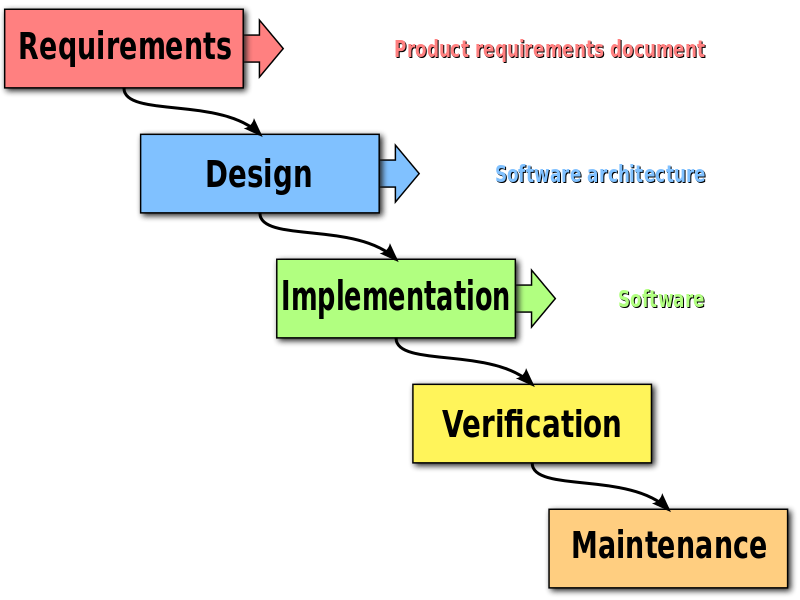
\includegraphics[scale=0.3]{./Images/Waterfall.png}
		\item[] We will use a sequential design process, used in software development processes, in which progress is seen as flowing steadily downwards through the phases of: 
		\begin{itemize}
			\item conception 
			\item initiation
			\item analysis
			\item design
			\item construction
			\item testing
			\item production/implementation
			\item maintenance
		\end{itemize}		 % Insert content here
		\item[] This is also known as the waterfall methodology.
	\end{itemize}
	
	\item Potential Technologies
	%(Potentially the technologies your team intends to use for the project (as far as these are not prescribed by the client))
	\begin{itemize}
		\item[] The technologies we plan to use are:
		\begin{itemize}
			\item On the Cloud Server
			\begin{itemize}
				\item NodeJS
				\item MongoDB for the database
				\item AngularJS for the client MVC framework
				\item OpenLayers 3 for the mapping of the locations of trackers
			\end{itemize}
			\item On the Gateway
			\begin{itemize}
				\item Arduino Platform
				\item Serial GSM Modules
				\item WebSockets for communication to server
				\item Bluetooth 4.0 (BLE) Receiver
				\item Serial GPS used for gateway positioning
			\end{itemize}
			\item On the Tracker
			\begin{itemize}
				\item Bluetooth 4.0 (BLE Beacon) with TI Chip CC2540
			\end{itemize}
		\end{itemize}
	\end{itemize}
	
	\item Outcome of the Project
	%(What the client will receive from you at the end of the project)
	\begin{itemize}
		\item The developed gateway/tracker application should include the following:
		\begin{itemize}
			\item[o] BLE communication
			\item[o] Socket Communication to the server
			\item[o] Positioning of trackers in range
			\item[o] GSM Connectivity
			\item[o] GPS Positioning
			\item[o] Rugged/Weather-proof containers
		\end{itemize}
		\item The developed alerting system should include the following:
		\begin{itemize}
			\item [o] SMS Notifications
			\item [o] Email Alerts
			\item [o] Local Buzzer Alerts
		\end{itemize}
		\item The developed web server application should include the following:
		\begin{itemize}
			\item [o] User friendly GUI
			\item [o] The ability to check the last location and the movement of trackers
			\item [o] The ability to specify who should have access to the client GUI and which trackers
		\end{itemize}
	\end{itemize}
	
\end{itemize}
